% Encoding: UTF-8
% kdtree.tex
% revised 10/12/2009
% $Header: acmtr.tex,v 1.5 2/14/96 11:07:57 boyland Exp $

\documentclass[acmjacm]{acmtrans2m}

\let\mycounter\setcounter

%&t&{\tt #}&
%&v&\verb|#|&

\acmVolume{2}
\acmNumber{3}
\acmYear{09}
\acmMonth{12}

\usepackage[utf8]{inputenc}
\usepackage{graphicx}
\usepackage{amsmath}
\usepackage{algorithmic}
\usepackage{algorithm}
\usepackage{url}
\usepackage{subfigure}


\newcommand{\BibTeX}{{\rm B\kern-.05em{\sc i\kern-.025em b}\kern-.08em
    T\kern-.1667em\lower.7ex\hbox{E}\kern-.125emX}}
\newcommand{\titulo}{Adaptive Load Balancing for MMOG servers using kd-trees}
\newcommand{\autores}{Carlos Eduardo B. Bezerra, João L. D. Comba and Cláudio F. R. Geyer}
\newcommand{\sbgamesaward}{(SBGames'09 awarded paper)}
\newcommand{\figurecaption}{Figure}

%\markboth{Leslie Lamport et al.}{Preparing Articles for the ACM}
\markboth{Carlos Eduardo Benevides Bezerra et al. \sbgamesaward{}}{\titulo{} \sbgamesaward{}}

\title{\titulo{}\\ \large{(invited extended version of the 2009 SBGames paper)}}
\author{CARLOS EDUARDO B. BEZERRA, JOÃO L. D. COMBA and CLÁUDIO F. R. GEYER\\Universidade Federal do Rio Grande do Sul}


\begin{abstract}
In Massively Multiplayer Online Games (MMOGs) there is a great demand for high bandwidth connections with irregular access patterns. Such irregular demand is due to the fact that players, which can vary from few hundreds to several tens of thousands, often occupy the virtual environment of the game in different ways with varying densities. Therefore, there is a great need for decentralized architectures with multiple servers that employ load balancing algorithms to manage regions of the virtual environment. In such systems, each player only connects to the server that manages the region where his avatar is located, whereas each 	server is responsible for mediating the interaction between all pairs of players connected to it. Devising the proper load balancing algorithm to take into account spatial and variable occupation is a challenging problem, which requires adaptive (and possibly dynamic) partitioning of the virtual environment. In this work, we propose the use of a kd-tree for partitioning the game environment into regions, and dynamically adjust the resulting subdivision based on the distribution of avatars in the virtual environment. We compared our algorithm to competing approaches found in the literature and show that our algorithm performed better in most aspects we analyzed.


%MMOGs (massively multiplayer online games) are applications that require high bandwidth connections to work properly. This demand for bandwidth is specially critical on the servers that host the game. This happens because the typical number of simultaneous participants in this kind of game varies from a few hundreds to several tens of thousands, and the server is the one responsible for mediating the interaction between every pair of players connected to it. To deal with this problem, decentralized architectures with multiple servers have been proposed, where each server manages a region of the virtual environment of the game. Each player, then, connects only to the server that manages the region where he is playing. However, to distribute the load among the servers, it is necessary to devise an algorithm for partitioning the virtual environment. In order to readjust the load distribution during the game, this algorithm must be dynamic. Some work has already been made in this direction, but with a geometric algorithm, more appropriate than those found in the literature, it should be possible to reduce the distribution granularity without compromising the rebalancing time, or even reducing it. In this work, we propose the use of a kd-tree for dividing the virtual environment of the game into regions, each of which being designated to one of the servers. The split coordinates of the regions are adjusted dynamically according to the distribution of avatars in the virtual environment. We compared our algorithm to some approaches found in the literature and the simulation results show that our algorithm performed better in most aspects we analyzed.

\end{abstract}

\category{C.2.4}{Computers Systems Organizations}{Computer-Communication Networks}%
[Distributed Systems]

\category{I.3.5}{Computing Methodologies}{Computer Graphics}[Computational Geometry and Object Modeling]

\terms{Algorithms, Management, Performance}

\keywords{distributed server, kd-trees, load balancing, MMOGs}


\newcommand{\misccite}[2]{#1. Available at: \textless#2\textgreater. Last time accessed: 24 jul. 2009}
\newcommand{\gamecite}[2]{\misccite{#1}{#2}}

\begin{document}


\setcounter{page}{1}



{\let\setcounter\mycounter
    \begin{bottomstuff}
    	Authors address: Programa de Pós-Graduação em Computação,
		Instituto de Informática, UFRGS,
		Caixa Postal 15064, 91501-970, Porto Alegre - RS - Brasil.
%		\newline
%		Start of a second footnote ...
    \end{bottomstuff}
}

\maketitle


\section{Introduction}

Massively Multiplayer Online Games (MMOGs) is a genre of computer games that demands high network bandwidth to allow
interaction among players. The main characteristic of MMOGs is the large number of players interacting simultaneously, which currently can reach up to tens of thousands \cite{schiele2007rpp}. Client-server architectures are often configured to allow communication among players, with the server intermediating the communication between each pair of players. To interact, each player sends commands to the server, which calculates the new game state and propagates it back to all players affected by the state change. This mechanism can lead to many state update messages sent by the server, which may be quadratic on the number of players in the worst case -- when all players interact with one another. Therefore, the cost of maintaining a centralized infrastructure like this is high when lots of players are connected, thus restricting the MMOG market to large companies with enough resources to pay the upkeep of the server.

To reduce this cost, several decentralized solutions have been proposed. Examples include peer-to-peer networks \cite{schiele2007rpp,rieche2007ppb,hampel2006ppa,elrhalibi2005abm,iimura2004zfg,knutsson2004pps} or distributed servers
\cite{ng2002msa,chertov:olb,lee2003sdl,assiotis2006dam},
which are composed of low-cost nodes connected through the Internet. Common to both approaches is the fact that the ``world'', or virtual environment of the game is divided into regions which are managed by a server (or a group of peers). Each region must not violate the network capacity of its respective server, and thus must not have more content than the load imposed on the corresponding server.

Players are assigned to servers based on their location. When an \emph{avatar} (representation of the player in the virtual environment) is located in a region, the player controlling that avatar connects to the server associated to that region. This server becomes responsible for processing the input from that player and for sending update messages in response. If a server becomes overloaded due to an excessive number of avatars in its region, one way to reduce its load is by repartitioning the virtual environment. Simply assigning players to different servers might not suffice, since they might not be able to absorb the excessive load.

Virtual environments are often divided into smaller cells, which are grouped into regions and distributed among servers. This approach has several limitations in its granularity due to cells of fixed size and position. More elaborate partitioning algorithms based in spatial data structures\cite{samet2005} allow better player distribution among different servers. In this work, we use a kd-tree to dynamically partition the virtual environment. When a server is overloaded, it triggers a load balancing algorithm, which changes the limits of each region by changing the split coordinates stored in the kd-tree. We validate our proposal with several simulations and compare the results to previous works that uses the cell division technique.

%The text is organized as follows: in section \ref{context}, some related works are described; in section \ref{sec:proposal}, the algorithm proposed here is presented in detail; in the sections \ref{sec:simul} and \ref{sec:result}, we present, respectively, the simulation details and its results and, in section \ref{sec:conc}, the conclusions of this work are presented.
%

\section{Related Work}
\label{context}

Different authors address the spatial partitioning of virtual environments in MMOGs for better distribution among multiple servers \cite{ahmed2008mol,bezerra2009lbs}. A simple approach is to partition the space into a static set of cells of fixed size and position, which are grouped into regions that are assigned to one of the servers (\figurecaption{} \ref{fig:cells}). When a server becomes overloaded, part of the load is transferred to another server.

\begin{figure}[!t]
	\centering
	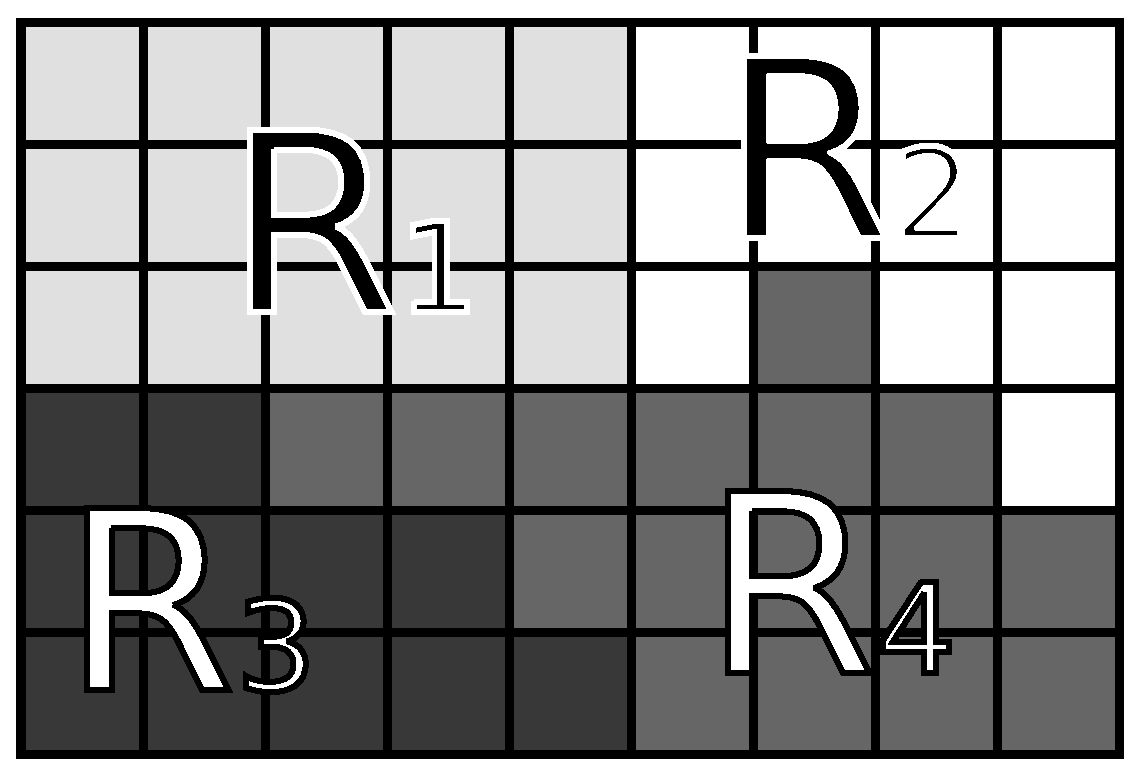
\includegraphics[width=0.4\linewidth]{images/macromicro}
	\caption{Division into cells and grouping into regions}
	\label{fig:cells}
\end{figure}

In the work of \cite{ahmed2008mol}, a cell-oriented load balancing model is proposed. Their algorithm first enumerates all clusters of cells that are managed by the overloaded server. The smallest cluster is found, and from this cluster is selected the cell with the least interaction with other cells on the same server -- the interaction between two cells A and B is defined by the authors as the number of pairs of avatars interacting with each other, one from A and the other from B. The selected cell is then transferred to the server
with the smallest load\footnote{considering ``load'' as the bandwidth used to send state updates to the players whose avatars are positioned in the cells managed by that server.}. This process is repeated until the server is no longer overloaded or there is no more servers capable of absorbing more load -- in this case, one option could be to reduce the frequency at which state update messages are sent to the players, as suggested by \cite{bezerra2008a3}.

\begin{figure}[!t]
	\centering
	\includegraphics[width=0.7\linewidth]{images/grafo}
	\caption{Graph representation of the virtual environment}
	\label{fig:graph}
\end{figure}

In \cite{bezerra2009lbs}, it is also proposed the division into cells. To perform the division, the environment is represented by a graph, where each vertex represents a cell (\figurecaption{} \ref{fig:graph}). Every edge in the graph connects two vertices representing neighboring cells. The weight of a vertex is the server's bandwidth used to send state updates to the players whose avatars are in the cell represented by that vertex. The interaction between any two cells defines the weight of the edge connecting the corresponding vertices. To form the regions, the graph is partitioned using a greedy algorithm: starting from the heaviest vertex, at each step it is added the vertex connected by the heaviest edge to any of the vertices already selected, until the total weight of the partition of the graph -- defined as the sum of the vertices' weights -- reaches a certain threshold related to the total capacity of the server that will receive the region represented by that partition of the graph.

This approach has a limited granularity distribution. If a finer granularity is desired, it is necessary to use smaller cells. This increases the number of vertices in the graph that represents the virtual environment and, consequently, the time required to perform load balancing. Also, the control message with the list of cells designated to each server becomes longer. A possibility to circumvent this problem relies on partitioning the virtual environment using spatial data structures \cite{bentley1975mbs}, for example
kd-trees or Binary Space Partitioning (BSP)-trees  
 (\figurecaption{} \ref{fig:bsp}).

Spatial data structures are widely used in Computer Graphics, and can be used to partition the virtual environments of MMOGs. There
is a vast literature on techniques that aim at creating spatial partitions with balanced ``loads''. In \cite{luque2005bpc}, the goal is to reduce the time needed to calculate collision detection between pairs of objects in a dynamic environment. A BSP-tree is used to distribute the objects in the scene. Objects that are in different partitions do not collide and there is no need to perform a complex collision test. It is proposed a dynamic readjustment of the tree as objects move, balancing their distribution on the leaf-nodes of the tree and, therefore, minimizing the time required to perform collision detection. Such ideas are used for load balancing among servers in MMOGs.

\begin{figure}[!t]
	\centering
	\subfigure[]{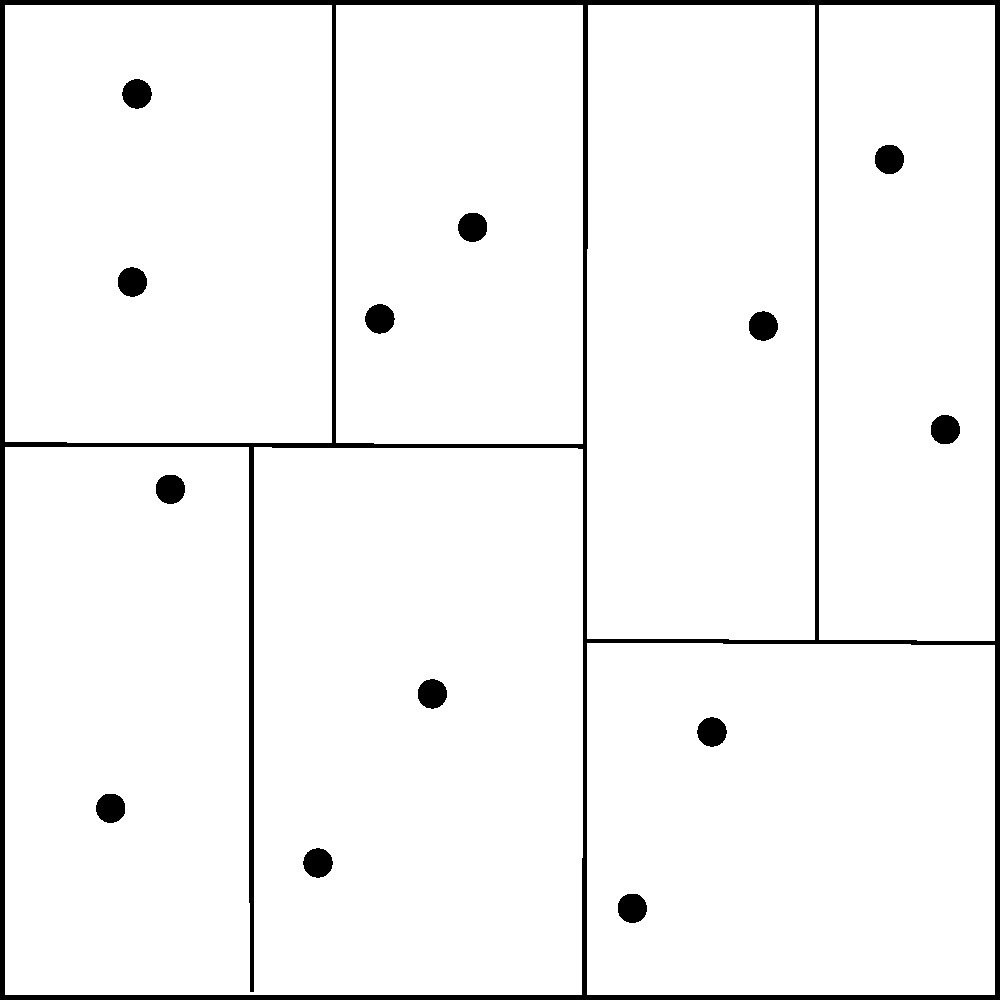
\includegraphics[width=0.3\linewidth]{images/kdtree2}}
	\subfigure[]{\includegraphics[width=0.3\linewidth]{images/bsp}}
	\caption{Space partitioning using a kd-tree (a) and a BSP tree (b).}
	\label{fig:bsp}
\end{figure}

\section{Proposed approach}
\label{sec:proposal}

In this section we describe our load balancing algorithm. The proposal is based on two criteria: first, we define the \textit{load} of a server as the bandwidth to send state updates to clients; and, second, the system should be considered heterogeneous (i.e. every server may have a different amount of available bandwidth). Since every player may interact to many others, the load on each server should be proportional to the bandwidth required to send state update messages to the players connected to it. This allows each player to receive state updates from many other players, leading to a quadratic total number of state update messages to be sent by the servers. Also, upload rates are usually lower than download rates. Since the number of commands received by a server grows linearly with the number of players, we consider only the upload bandwidth to send state updates, ignoring the download rate used by the servers to receive commands from clients.

As mentioned before, we propose the utilization of a data structure known as kd-tree to divide the environment of the game into regions. 
Despite having three-dimensional graphics, the vast majority of MMOGs (e.g. World of Warcraft \cite{worldofwarcraft}, Ragnarok \cite{ragnarok} and \mbox{Lineage II} \cite{lineage2} have a 2D simulated world -- cities, forests, swamps and points of interest in general. Therefore, we propose to use a 2D kd-tree.

Each node of the tree represents a region of the space defined by a coordinate used to split the space. Each of the two children of that node represents the two half-spaces obtained in the partitioning process. We alternate the splitting axis (in the case of two dimensions, the axes $x$ and $y$) at each level of the tree -- if the first level nodes store x-coordinates, the second level nodes store y-coordinates and so on. Every leaf node also represents a region of the space, but it does not store any split coordinate. Instead, it stores a list of the avatars present in that region. Finally, each leaf node is associated to a server of the game. When a server is overloaded, it triggers the load balancing, which uses the kd-tree to readjust the split coordinates that define its region, reducing the amount of content.

The nodes of the kd-tree also store two other values: capacity and load of the subtree. The load of a leaf node is equal to the load of the associated region. Similarly, the capacity of a leaf node corresponds to the network capacity of its associated server. For each non-leaf node, the load and capacity values correspond to the sum of those stored in its child nodes. The tree root stores, therefore, the total weight of the game and the total capacity -- upload bandwidth -- of the server system.

In the following sections, we will describe the construction of the tree, the calculation of the load associated with each server and the proposed balancing algorithm.

\subsection{Building the kd-tree}

The initial kd-tree is constructed in such way that it represents a balanced tree. Algorithm \ref{alg:buildtree} is used to create the tree, starting from instantiating a single root node which calls $node.build\_tree(0,0,n)$, where $n$ is the number of leaf nodes (corresponding to the number of servers, in our case).

\begin{algorithm}
\caption{node::build\_tree(id, level, n)}
\label{alg:buildtree}
\begin{algorithmic}
 \STATE $this.node\_id \leftarrow id$;
	\IF{id + $2^{level} \ge n$ }
		\STATE $left\_child \leftarrow NIL$;
		\STATE $right\_child \leftarrow NIL$;
		%\STATE return;
	\ELSE
		\STATE $left\_child \leftarrow$ new\_node();
		\STATE $left\_child.parent \leftarrow$ \textbf{this};
		\STATE $right\_child \leftarrow$ new\_node();
		\STATE $right\_child.parent \leftarrow$ \textbf{this};
		\STATE $left\_child$.build\_tree$(id, level + 1, n)$;
		\STATE $right\_child$.build\_tree$(id + 2^{level}, level + 1, n)$;
	\ENDIF
\end{algorithmic}
\end{algorithm}

\begin{figure}[!t]
	\centering
	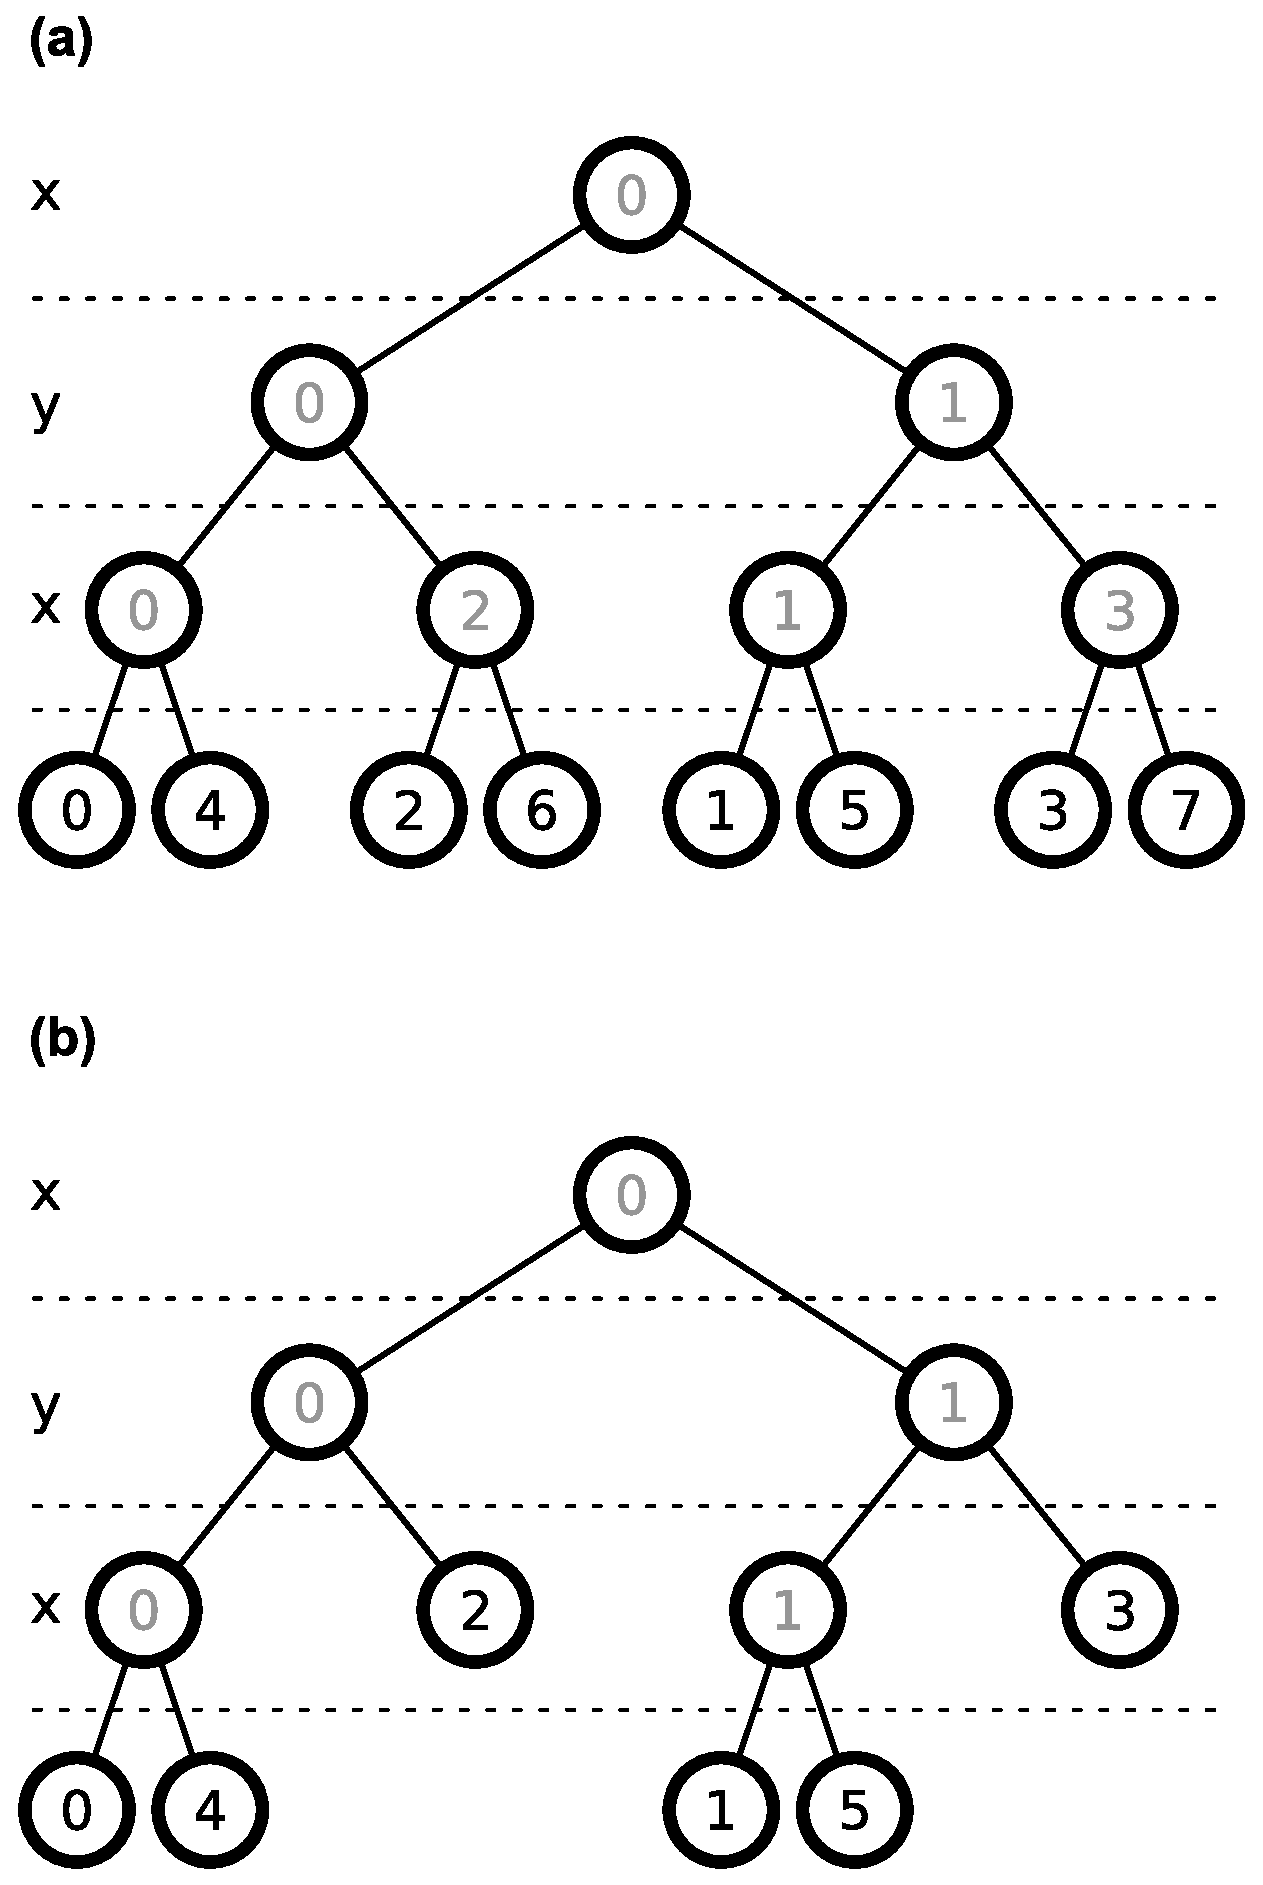
\includegraphics[width=\linewidth]{images/kdtree}
	\caption{Balanced kd-trees built with the described algorithm. (a) full (b) incomplete}
	\label{fig:kdtree}
\end{figure}

In Algorithm \ref{alg:buildtree}, $id$ is used to calculate whether each node has children or not. This allows to create a balanced tree where the difference between the number of leaf nodes in the two sub-trees of any given node is at most one. In \figurecaption{} \ref{fig:kdtree} (a), we have a full kd-tree formed with this simple algorithm and, in \figurecaption{} \ref{fig:kdtree} (b), an incomplete kd-tree with six-leaf nodes. As we can see, every node of the tree in (b) has two sub-trees whose number of leaf nodes differs by one in the worst case.

\subsection{Calculating the load of avatars and tree nodes}

The definition of the split coordinate for every non-leaf node of the tree depends on how the avatars will be distributed among regions. An initial idea might be to distribute players in a way such that the number of players on each server is proportional to its upload bandwidth. To calculate the split coordinate it is enough to sort the $n$ avatars based on their coordinates along the split axis ($x$ or $y$) and assign the first $n'$ avatars to the left child and the last $n - n'$ ones to the right child, where $n'$ and $n - n'$ are proportional to the capacity of the left and right child, respectively (\figurecaption{} \ref{fig:vector}). At each node, this operation cost $O(nlogn)$ due to sorting. Assigning all avatars to the root node and recursively executing this operation would have a complexity of $O(nlog^2n)$, as it must me repeated for each of the $O(logn)$ levels of the kd-tree.

\begin{figure}
  \centering
  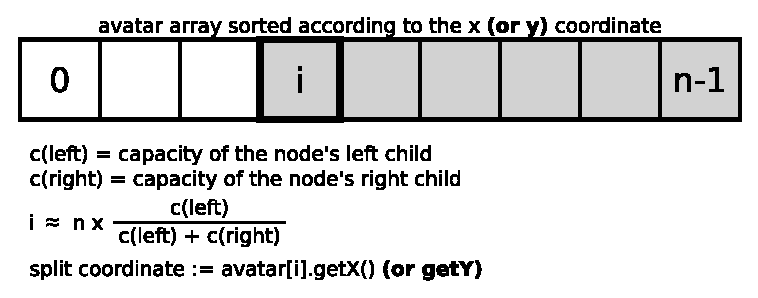
\includegraphics[width=0.8\linewidth]{images/vector}
  \caption{A load splitting considering only the number os avatars}
  \label{fig:vector}
\end{figure}

However, this distribution is not optimal since the load imposed by players depends on how they are interacting with one another. For example, if the avatars of two players are distant from each other, there will be probably no interaction between them and, therefore, the server need to update the outcome of their own actions. In this case, the growth in the number of messages is linear with the number of players. On the other hand, if the avatars are close to each other, each player should be updated not only about the outcome of their actions but also about the actions of every other player -- in this case, the number of messages may grow quadratically with the number of players \mbox{(\figurecaption{} \ref{fig:load})}. For this reason, it is not enough to consider only the number of players when dividing them among servers.

\begin{figure}
  \centering
  
\includegraphics[width=0.8\linewidth]{images/carga}
  \caption{Relation between avatars and load}
  \label{fig:load}
\end{figure}

A more appropriate way to divide the avatars is by considering the load imposed by each one on the server. A brute-force method for calculating the load is to get the distance separating each pair of avatars and, based on their interaction, and calculate the number of messages that each player should receive by unit of time. This approach has complexity $O(n^2)$. One way to speedup this
calculation is to sort avatars according to their coordinates on the axis used to divide the space in the kd-tree.

For this, two nested loops are used to sweep the avatars array, where each of the avatars contains a $load$ variable initialized with zero. As the vector is sorted, the inner loop starts at the smallest index that indicates that no avatar $a_j$ has relevance to the one referenced in the outer loop, $a_i$. It uses a variable $begin$, with initial value of zero: if the coordinate of $a_j$ is smaller than $a_i$, with a difference greater than the maximum view range of the avatars, the variable $begin$ is incremented. For every $a_j$ which is at a distance smaller than the maximum view range, the $load$ of $a_i$ is increased according to the relevance\footnote{The relevance of an object to an avatar may be used to define how many state update messages its player must receive about that object per time unit \cite{bezerra2008a3} -- for that matter, avatars are also considered objects. One possible approach is to define the relevance of an object to an avatar as their proximity in the virtual environment.} of $a_j$ to $a_i$. When the inner loop reaches an avatar $a_j$, such that its coordinate is greater than $a_i$, with a difference greater than the view range, the outer loop moves immediately to the next step, incrementing $a_i$ and setting the value of $a_j$ to that stored in $begin$ (\figurecaption{} \ref{fig:sweep}).

To evaluate the complexity of the algorithm, we refer to $width$ as the length of the virtual environment along the axis used for the splitting; $radius$ as the maximum view range of the avatars, and $n$, the number of avatars. The number of relevance calculations, assuming that avatars are uniformly distributed in the virtual environment is \mbox{$O(m \times n)$}, where $m$ is the number of avatars compared in the internal loop, i.e. \mbox{$m = \frac{2 \times radius \times n}{width}$}. Sorting avatars along one of the axes takes $O(nlogn)$. Although it is still quadratic, the execution time is reduced significantly, depending on the size of the virtual environment and on the view range of the avatars. The algorithm could also sort each set of avatars $a_j$ which are closer (in one of the axes) to $a_i$ according to the other axis and, again, perform a sweep eliminating those which are too far away, in both dimensions. The number of relevance calculations would be \mbox{$O(p \times n)$}, where $p$ is the number of avatars closer to $a_i$, considering the two axes of coordinates, i.e. \mbox{$p = \frac{(2 \times radius)^2 \times n}{width \times height}$}. In this case, $height$ is the extension of the environment in the second axis taken as reference. Although there is a considerable reduction of the number of relevance calculations, it does not compensate the time spent in sorting the sub-array of avatars selected for each $a_i$. Adding up all the time spent on sorting operations, we obtain a complexity of: \mbox{$O(nlogn + n \times mlogm)$}.

\begin{figure}
  \centering
  \includegraphics[width=0.8\linewidth]{images/sweep}
  \caption{Sweep of the sorted array of avatars}
   \label{fig:sweep}
\end{figure}

The load generated by each avatar is used to define the load on each leaf node, This can be done because each avatar is located in a region, which is represented by a leaf node. The load is calculated recursively for the other nodes of the kd-tree. As mentioned before, each leaf node is assigned a server and a region of the virtual environment. When the load of a leaf node is equal to the server's bandwidth used to send state updates to the players controlling the avatars located in its associated region, the load of each leaf node is equal to the sum of the weights of all avatars located in their respective regions.

\subsection{Dynamic load balancing}

The overloading of a sever  indicates that part of its load must be assigned to a different server. To accomplish this, the overloaded server collects data -- list of avatars, their positions and loads -- from other servers and, using the kd-tree, adjusts the split coordinates of the regions.

Every server maintains an array of avatars located in its respective region, sorted by the $x$ coordinate. Also, each element of the array stores a pointer to a linked list that ordered by the $y$ coordinated of avatars (\figurecaption{} \ref{fig:vectorxlisty}). Using a local sorted avatar list on each server, the time required for balancing the load is reduced, since there is no need for the server to sort again the avatar lists sent by other servers. It only needs to merge all avatars lists received from the other servers in an unique list, used to define the limits of the regions, which is done by changing the split coordinates used to partition the space.

\begin{figure}
  \centering
  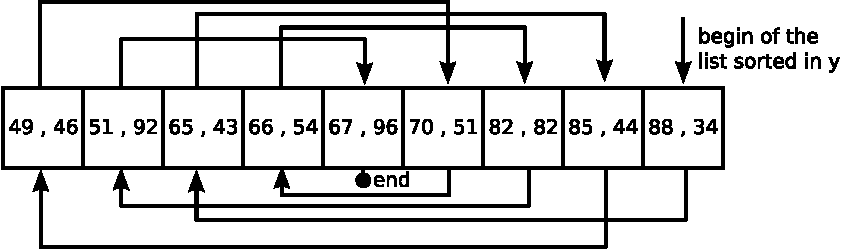
\includegraphics[width=0.9\linewidth]{images/vectorxlisty}
  \caption{Avatar array sorted by x, containing a list sort by y}
   \label{fig:vectorxlisty}
\end{figure}

After the overloaded server initiates the rebalance, it runs an algorithm that traverses upward the kd-tree starting from the leaf node associated to the overloaded server. This traversal moves one level up at each step until it finds an ancestor node with a capacity greater than or equal to the load. At each step, the algorithm visits a node which has a sub-tree containing other servers (leaf nodes), whose avatar list, load value and capacity value are probably unknown or outdated to the initiating server. A request is sent to these servers, requiring the current avatar list and the current values of load and capacity (\figurecaption{} \ref{fig:ancestors}). With these data, and the initiating server's own list of avatars and values of load and capacity, the algorithm can calculate the load and capacity of the ancestral nodes visited in the kd-tree, which are not known beforehand -- these values are sent on-demand to save up some bandwidth of the servers and to keep the system scalable.

\begin{figure}
  \centering
  \includegraphics[width=0.8\linewidth]{images/ancestors}
  \caption{Search for an ancestor node with enough resources}
   \label{fig:ancestors}
\end{figure}

Reaching an ancestral node with capacity greater than or equal to the load -- or the root of the tree, if no such node is found -- the initiating server adjusts the split coordinates of the kd-tree nodes. For each node, it sets the split coordinate in a way such that the avatars are distributed according to the capacity of the node's children. For this, it is calculated the load fraction that should be assigned to each child node. The avatar list is then swept, stopping at the index $i$ such that the total load of the avatars before $i$ is approximately equal to the value defined as the load to be designated to the left child of the node whose split coordinate is being calculated (\figurecaption{} \ref{fig:balancenode}). The children nodes have also, in turn, their split coordinates readjusted recursively, so that they are checked for validity -- the split coordinate stored in a node must belong to the region defined by its ancestors in the kd-tree -- and readjusted to follow the balance criteria defined.

\begin{figure}
  \centering
  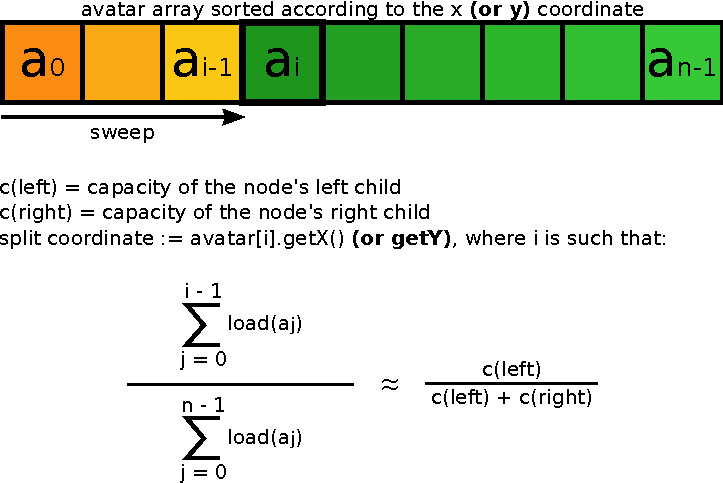
\includegraphics[width=0.8\linewidth]{images/balancenode}
  \caption{Division of an avatar list between two brother nodes}
   \label{fig:balancenode}
\end{figure}

As the avatar lists received from the other servers are already sorted along both axes, it is enough to merge these structures with the avatar list of the server which initiated the rebalance. Assuming that each server already calculated the weight of each avatar managed by it, the rebalance time is  $O(nlogS)$, where $n$ is the number of avatars in the game and $S$ is the number of servers. The communication cost is $O(n)$, caused by the sending of data related to $n$ avatars. The merging of all avatar lists has $O(n)$ complexity, for the avatars were already sorted by the servers. At each level of the kd-tree, $O(n)$ avatars are swept in the worst case, in order to find the $i$ index whose avatar's coordinate will be used to split the regions defined by each node of the tree (\figurecaption{} \ref{fig:balancenode}). As this is a balanced tree with $S$ leaf nodes, it has a height of $\lceil logS \rceil$, explaining the $O(nlogS)$ overall complexity of the rebalancing algorithm described.

\section{Simulations}
\label{sec:simul}

A virtual environment with several moving avatars was simulated to evaluate the proposed dynamic load balancing algorithm, 
 Starting from a random point in the environment, each avatar moves according to the random waypoint model \cite{bettstetter2004spr}. To force a load imbalance and stress the algorithms tested, we defined some \emph{hotspots} -- points of interest to which the avatars moved with a higher probability than to other parts of the map. This construction allows for a high concentration of avatars in some areas. Although the model used to control player movement is not very realistic in terms of the way the players move their avatars in real games, it was only used to verify the load balance algorithms simulated. For each algorithm tested, we simulated scenarios with 750 and 1500 players, with and without hotspots. In the hotspot cases, we simulated different probabilities (70\% and 90\%) of each player selecting one of the hotspots as the next waypoint to move. Combining all these parameters, we simulated six different scenarios for each algorithm -- \figurecaption{} \ref{fig:scenarios} illustrates each situation.

\begin{figure}
  \centering
  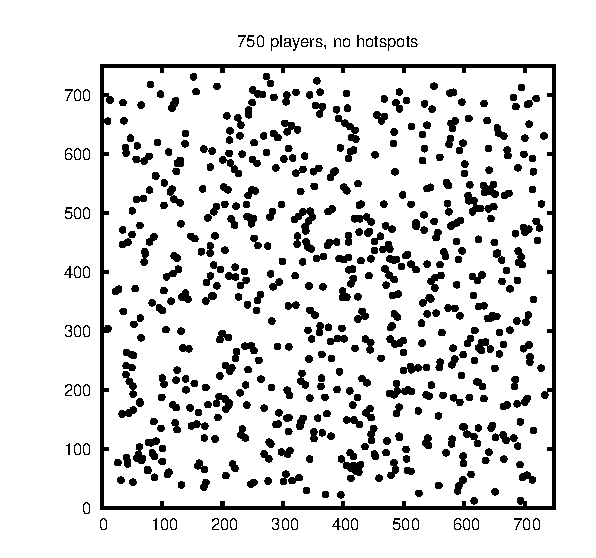
\includegraphics[width=0.49\linewidth]{data/750players_prob0/avatarsdistribution}
  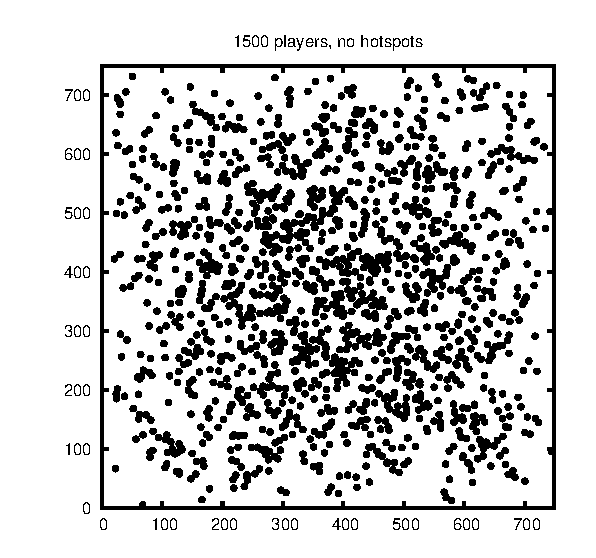
\includegraphics[width=0.49\linewidth]{data/1500players_prob0/avatarsdistribution}
  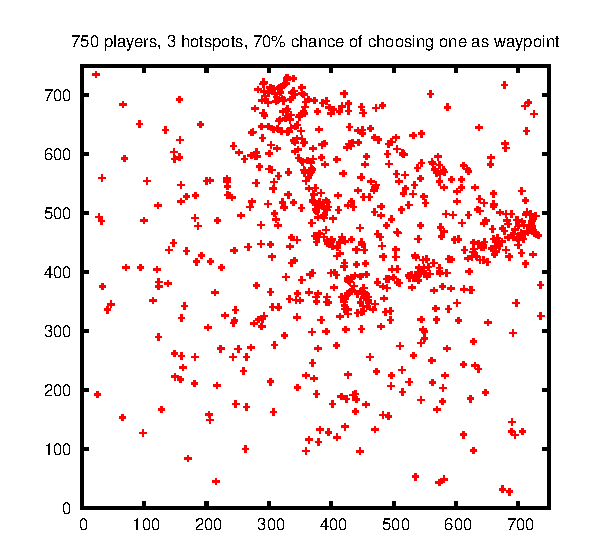
\includegraphics[width=0.49\linewidth]{data/750players_prob70/avatarsdistribution}
  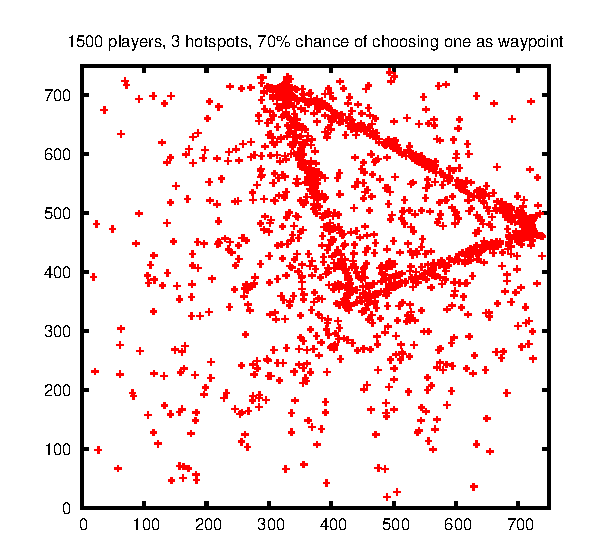
\includegraphics[width=0.49\linewidth]{data/1500players_prob70/avatarsdistribution}
  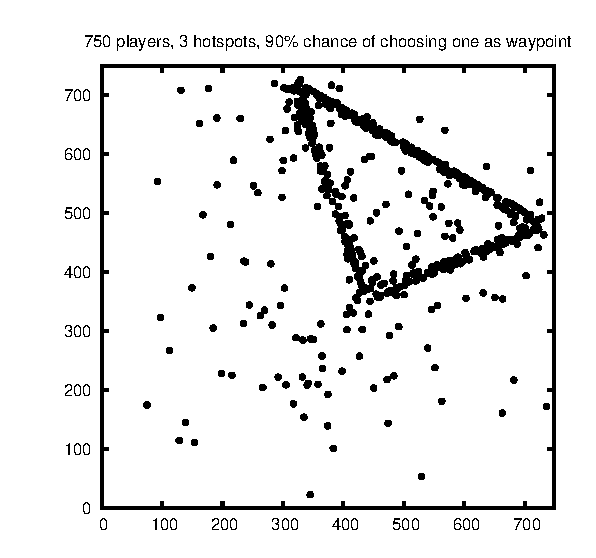
\includegraphics[width=0.49\linewidth]{data/750players_prob90/avatarsdistribution}
  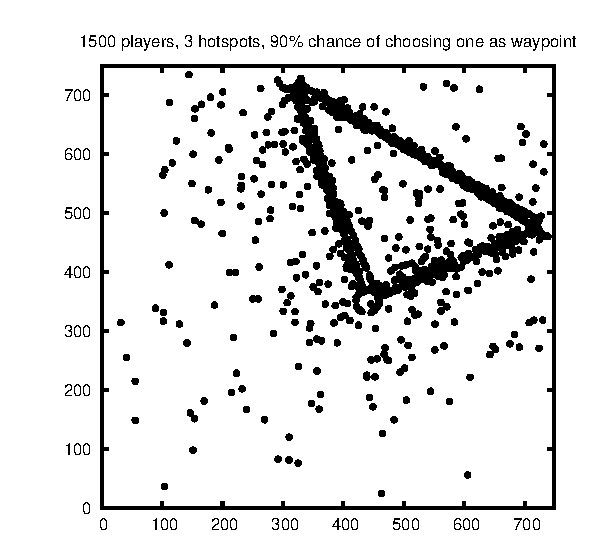
\includegraphics[width=0.49\linewidth]{data/1500players_prob90/avatarsdistribution}
  \caption{Scenarios in which the algorithms were simulated}
   \label{fig:scenarios}
\end{figure}

The reason why we chose three kinds of avatar distribution -- no hotspots, mildly concentrated around hotpots (70\%) and densely concentrated (90\%) -- was because we wanted to make realistic simulations. In most commercial MMOGs, there are points of interest, like towns and dungeons. Players wander throughout the virtual environment of the game, looking for adventure and treasures, going to some dungeon and coming back to town once in a while -- therefore, creating a mildly concentrated avatar population around these places. Frequently the game company creates special game events that attract most players to some locations in the game world, like a very powerful monster invading a town or a very rare and valuable treasure in a dungeon, creating a population density in these areas much higher than usual -- case to which the heavily concentrated simulation scenario refers. However, it is very uncommon to have absolutely no hotspots in a real MMOG, but this case was also simulated in order not only to cover this kind of no-hotspot situation, but also for its results to serve as a reference to the results of the scenarios with hotspots.

The proposed approach was compared to the ones presented in section \ref{context}. However, it is important to observe that the model employed by \cite{ahmed2008mol} considers hexagonal cells, while in our simulations we used rectangular cells. Furthermore, the authors considered that there is a transmission rate threshold, which is the same for all servers in the system. As we assume a heterogenous system, their algorithm was simulated considering that each server has its own transmission rate threshold, depending on the upload bandwidth available for each one of them. However, we kept what we consider the core idea of the authors' approach, which is the selection of the smallest cell cluster managed by the overloaded server, then choosing from this cluster the cell with the lowest interaction with other cells of the same server, and finally the transferring of this cell to the least loaded server. Besides Ahmed's algorithm, we also simulated some of the ones proposed in \cite{bezerra2009lbs} -- Progrega and BFBCT.

The simulated virtual environment consisted of a two-dimensional space, with 750 moving avatars, whose players were divided among eight servers ($S_1, S_2, ..., S_8$), each of which related to one of the regions determined by the balancing algorithm. For the cell-oriented approaches simulated, the space was divided into a \mbox{15 $\times$ 15} cell grid -- or 225 cells. The \textbf{capacity}\footnote{The network capacity is a value proportional to the upload bandwidth of each simulated server.} of each server $S_i$ was equal to $i \times 20000$, forming a heterogeneous system. This heterogeneity allowed us to evaluate the load balancing algorithms simulated according to the criterion of proportionality of the load distribution on the servers.

In addition to evaluate the algorithms according to the proportionality of the load distribution, it was also considered the number of player migrations between servers. Each migration involves a player connecting to the new server and disconnecting from the old one. This kind of situation may occur in two cases: the avatar moved, changing the region in which it is located and, consequently, changing the server to which its player is connected; or the avatar was not moving and still its player had to migrate to a new server. In the latter case, obviously the player's transfer was due to a rebalancing. An ideal balancing algorithm performs the load redistribution requiring the minimum possible number of player transfers between servers, while keeping the load on each server under (or proportional to) its capacity.

Finally, the inter-server communication \textbf{overhead}\footnote{The inter-server communication overhead here represents the amount of bandwidth wasted by the servers when intermediating interactions of players who are in different regions. This happens because, in each of these interactions, there is more than one intermediate server.} %, and thus they need to exchange messages.}
was also evaluated. It occurs when two players are interacting, but each one of them is connected to a different server. Although the algorithm proposed in this work does not address this problem directly, it would be interesting to evaluate how the load distribution performed by it influences the communication between the servers.

\section{Results}
\label{sec:result}

\begin{figure}[!t]
	\centering
	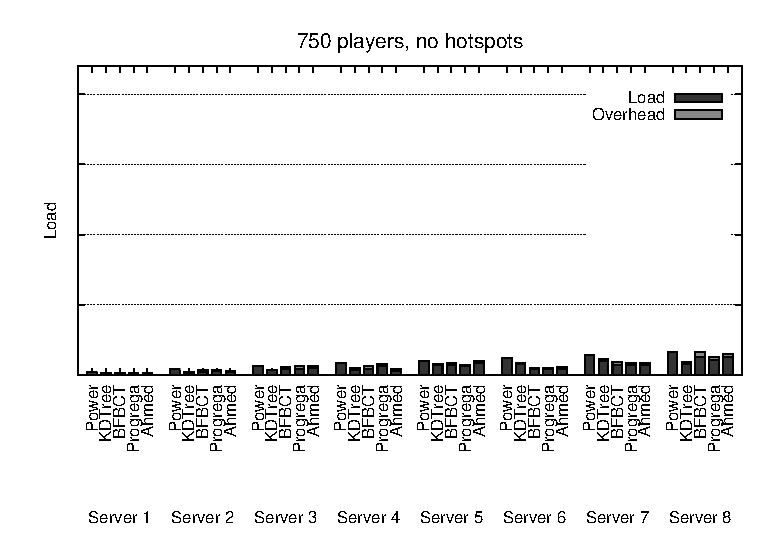
\includegraphics[width=0.495\linewidth]{data/750players_prob0/distribution_750_0}
	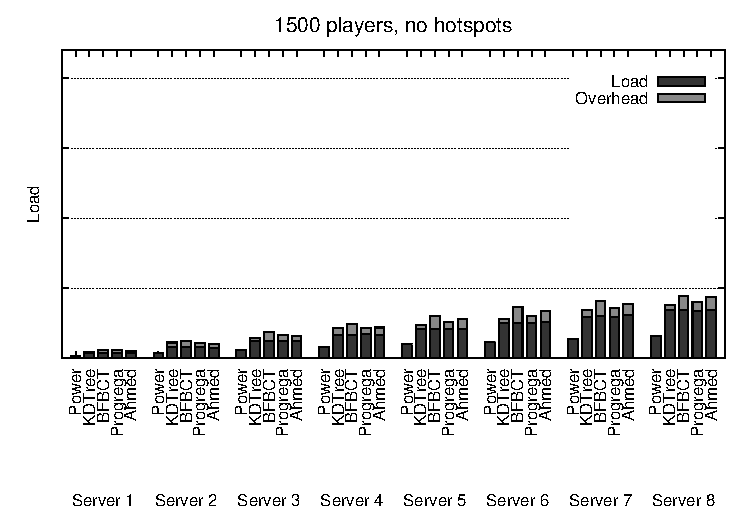
\includegraphics[width=0.495\linewidth]{data/1500players_prob0/distribution_1500_0}
	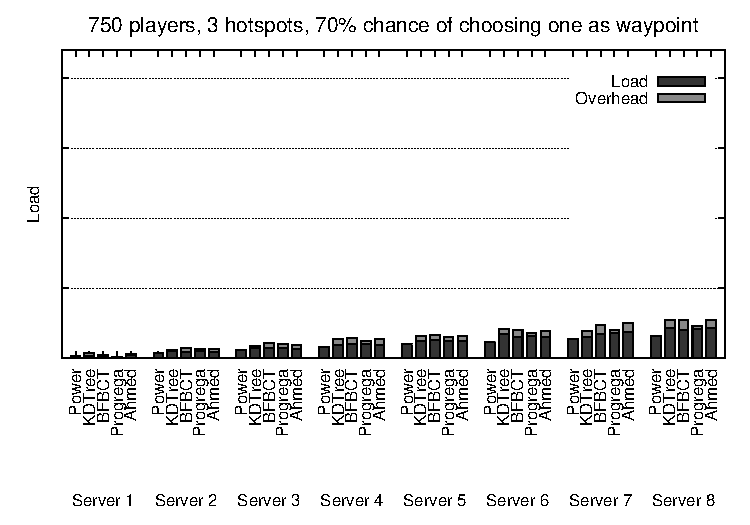
\includegraphics[width=0.495\linewidth]{data/750players_prob70/distribution_750_70}
	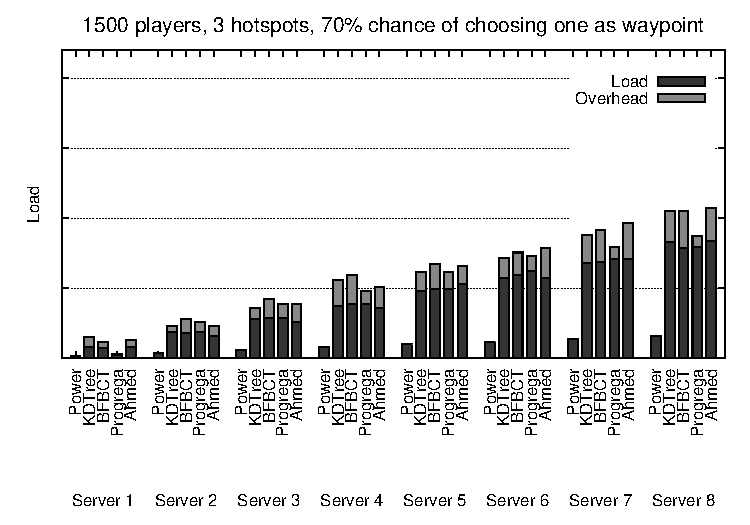
\includegraphics[width=0.495\linewidth]{data/1500players_prob70/distribution_1500_70}
	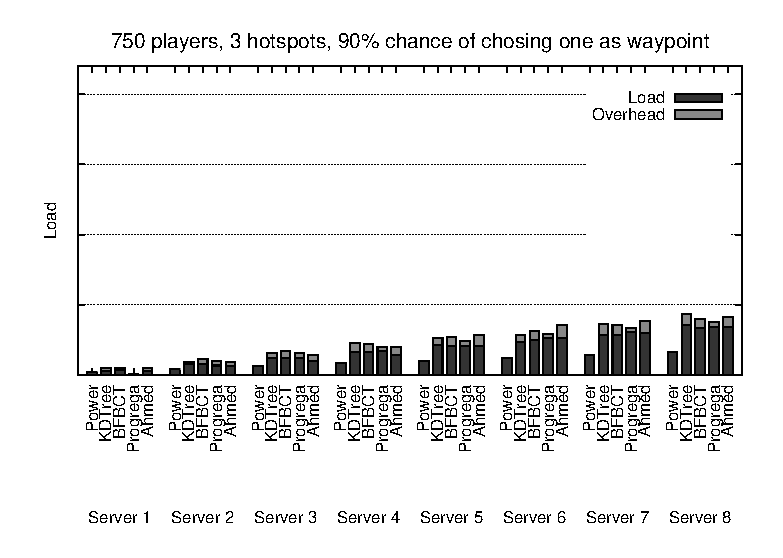
\includegraphics[width=0.495\linewidth]{data/750players_prob90/distribution_750_90}
	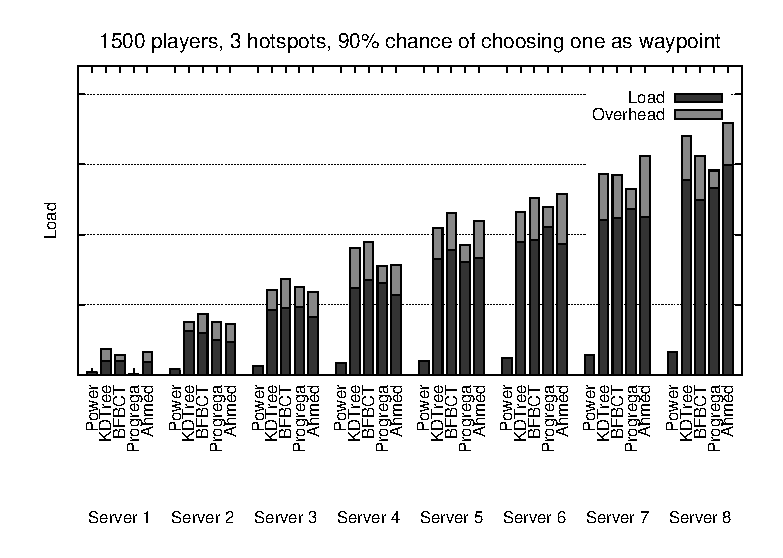
\includegraphics[width=0.495\linewidth]{data/1500players_prob90/distribution_1500_90}

	\caption{Average load on each server in each scenario}
	\label{fig:distribution}
\end{figure}

\figurecaption{} \ref{fig:distribution} presents the average load (plus the inter-server communication overhead) on each server, for each algorithm tested. The first two graphics show the values in a situation without hotspots and so they present a lower total load. The next two graphics, in turn, present the load distribution when the players tend to move towards one of the hotspots, increasing the number of interactions and, thus, the load on the servers. Finally, the two bottom graphics show the load on the servers when not only there are hotspots, but also the probability of a player moving to one of them is considerably high (90\%). Although this is not the worst case -- all players interacting with one another --, the load increase on the servers is significant.

We can see that all algorithms have met the objective of keeping the load on each server lower than or proportional to its capacity, in all situations considered. When the server system is overloaded (as in every graphic of \figurecaption{} \ref{fig:distribution}, apart from the first), it is demonstrated that all the algorithms managed to dilute -- in a more or less proportional manner -- the load excess on the servers. It is important to observe, however, that the load shown in the figure is only theoretical. Each server will perform some kind of ``graceful degradation'' in order to keep the load under its capacity. For example, the update frequency might be reduced and access to the game could be denied for new players attempting to join, which is a common practice in most MMOGs.

\begin{figure}[!t]
	\centering
	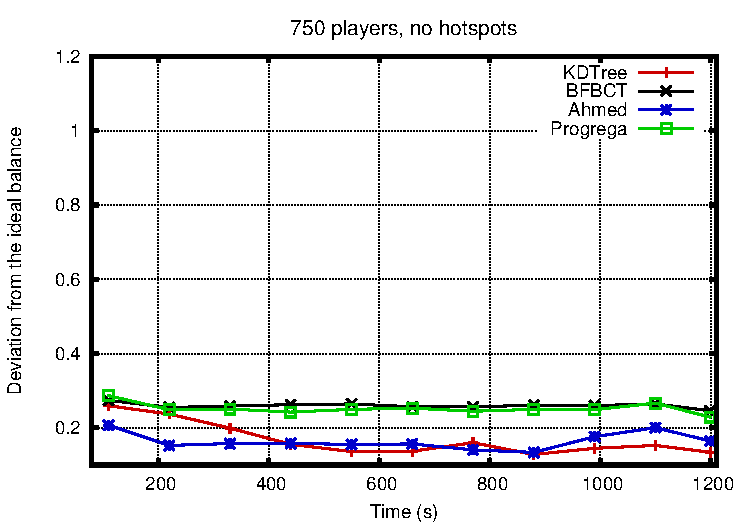
\includegraphics[width=0.49\linewidth]{data/750players_prob0/usagedeviation}
	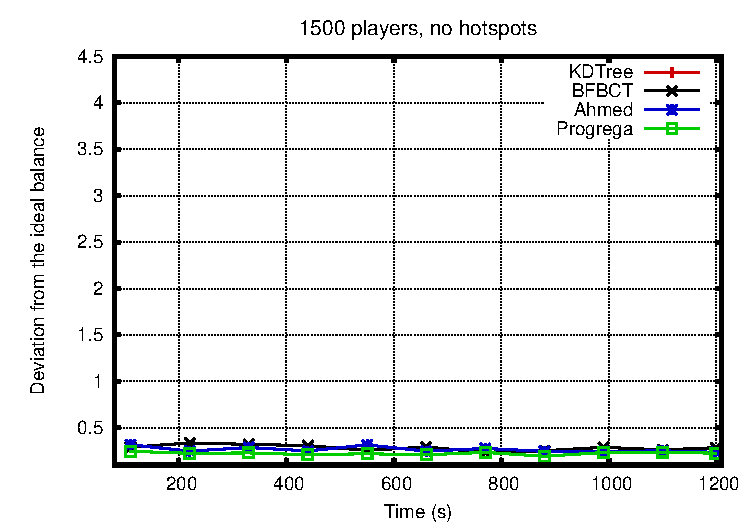
\includegraphics[width=0.49\linewidth]{data/1500players_prob0/usagedeviation}
	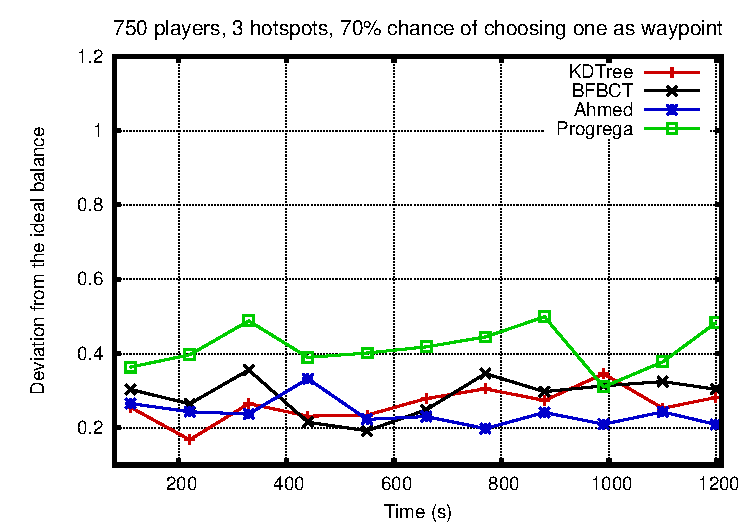
\includegraphics[width=0.49\linewidth]{data/750players_prob70/usagedeviation}
	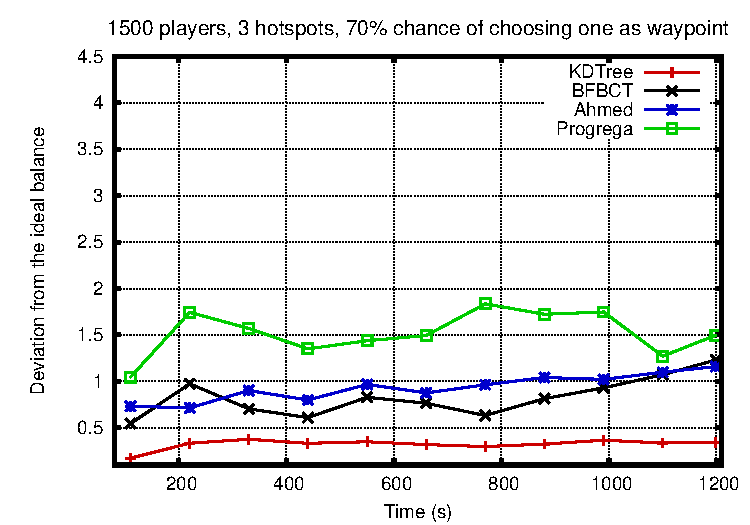
\includegraphics[width=0.49\linewidth]{data/1500players_prob70/usagedeviation}
	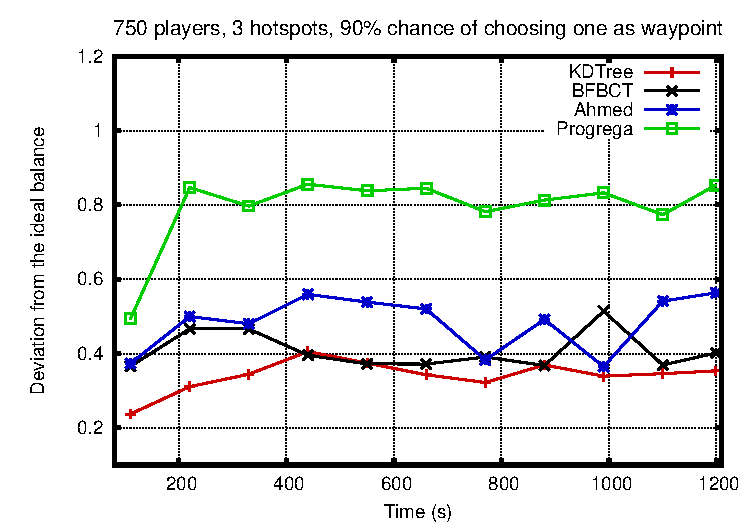
\includegraphics[width=0.49\linewidth]{data/750players_prob90/usagedeviation}
	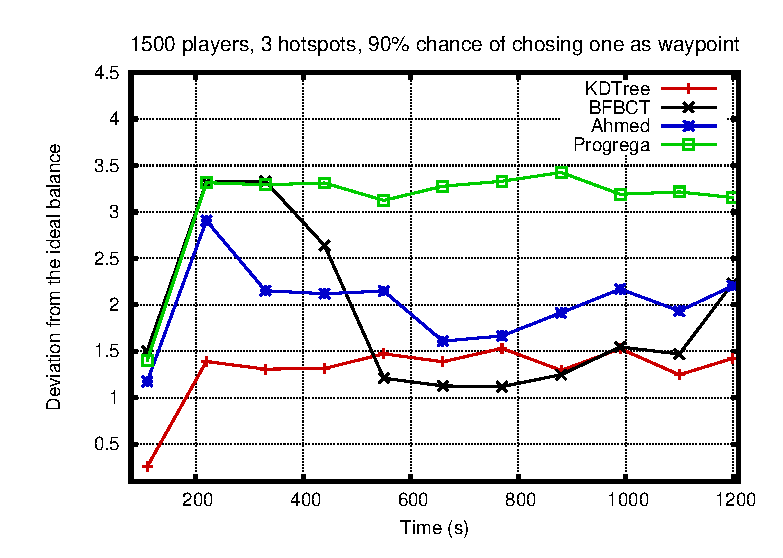
\includegraphics[width=0.49\linewidth]{data/1500players_prob90/usagedeviation}

	\caption{Average deviation of the ideal balance of the servers in each scenario}
	\label{fig:usagedeviation}
\end{figure}

In \figurecaption{} \ref{fig:usagedeviation}, it is shown how much the balance generated by each algorithm deviates from an ideal balance -- i.e., how much on the average the load on the servers deviate from a value exactly proportional to the capacity of each one of them -- over time. It is possible to observe that, at least in three of the situations of greatest overload, the algorithm that uses the kd-tree has the least deviation. This is the due to the fine granularity of its distribution, which, unlike the other approaches tested, is not limited by the size of a cell. In the situations of heavy overload, the algorithm that uses the kd-tree is particularly effective, because rebalance is needed. In a situation where the system has enough resources, the proportionality of the distribution is not an important issue: it is enough that each server manages a load smaller than its capacity.

\begin{figure}[!t]
	\centering
	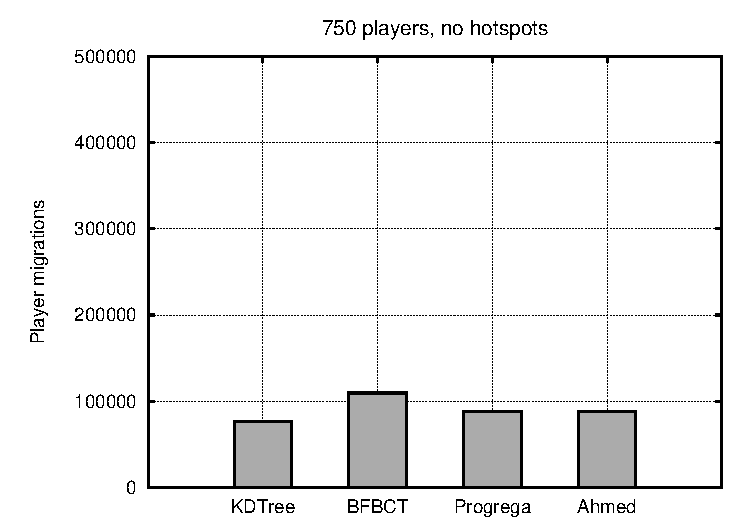
\includegraphics[width=0.49\linewidth]{data/750players_prob0/migrations}
	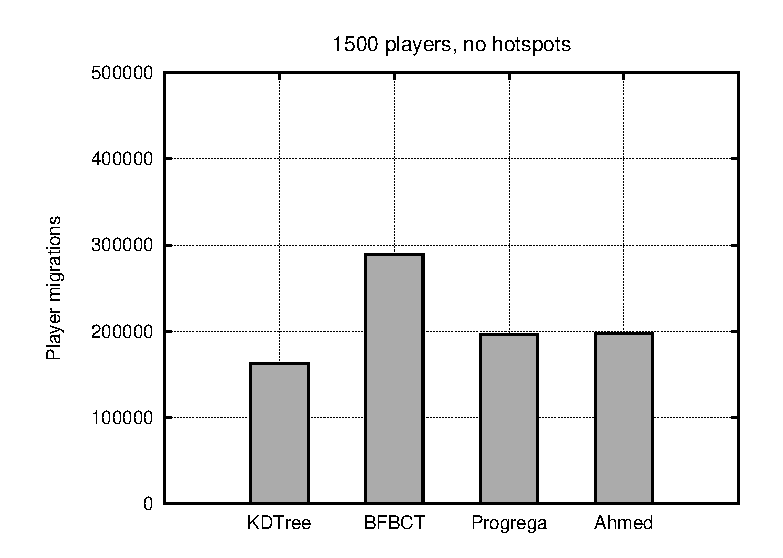
\includegraphics[width=0.49\linewidth]{data/1500players_prob0/migrations}
	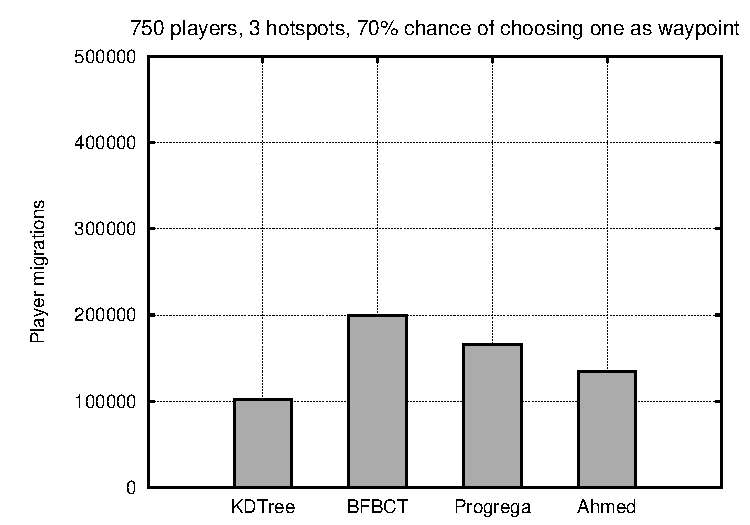
\includegraphics[width=0.49\linewidth]{data/750players_prob70/migrations}
	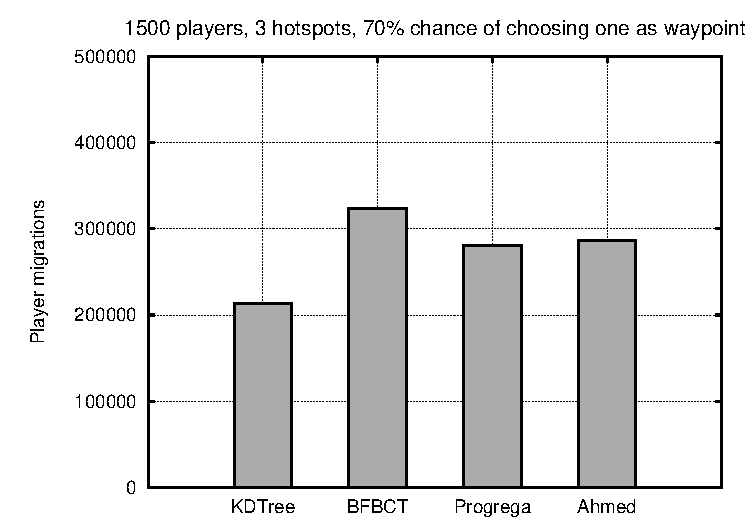
\includegraphics[width=0.49\linewidth]{data/1500players_prob70/migrations}
	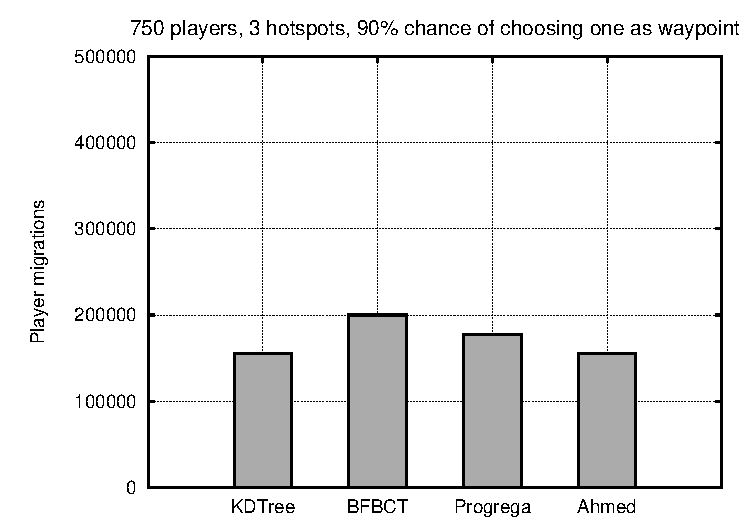
\includegraphics[width=0.49\linewidth]{data/750players_prob90/migrations}
	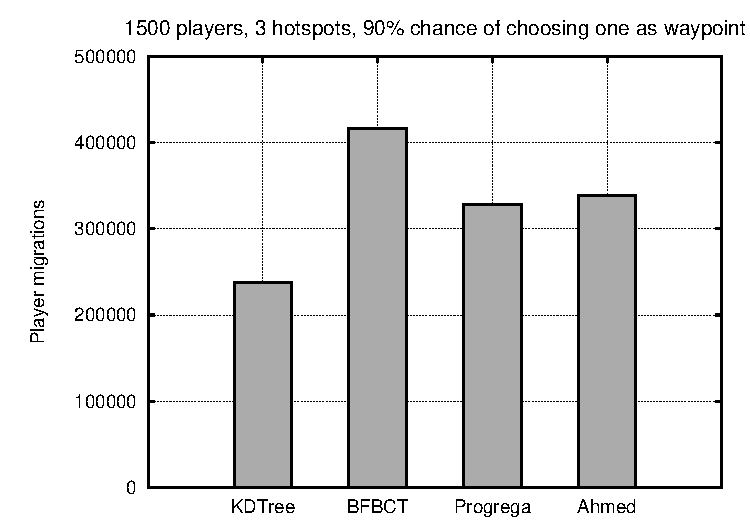
\includegraphics[width=0.49\linewidth]{data/1500players_prob90/migrations}
	\caption{Player migrations between servers in each scenario}
	\label{fig:migrations}
\end{figure}

Regarding player migrations between servers, the proposed approach not only performed considerably better than the others (\figurecaption{} \ref{fig:migrations}), as it also demonstrated a greater scalability, increasing its advantage over the other algorithms as the simulated scenario became more heavily loaded. This is due, in the first place, to the fact that the regions defined by the leaf nodes of the kd-tree are necessarily contiguous, and each server was linked to only one leaf node. An avatar moving across an environment divided into very fragmented regions constantly crosses the borders between these regions and causes, therefore, its player to migrate from server to server repeatedly. Another reason for this result is that each rebalancing executed with the kd-tree gets much closer to an ideal distribution than the cell-based algorithms -- again, thanks to the finer granularity of the kd-tree based distribution --, requiring less future rebalancing and, thus, causing fewer player migrations.

\begin{figure}[!t]
	\centering
	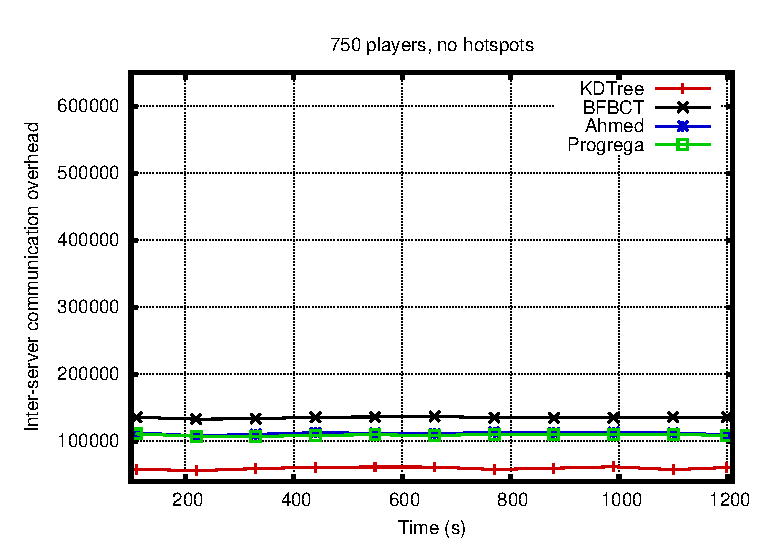
\includegraphics[width=0.49\linewidth]{data/750players_prob0/overhead}
	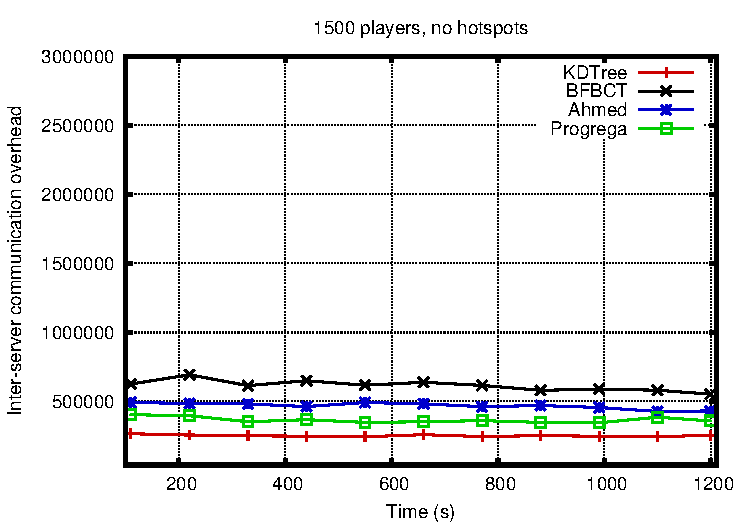
\includegraphics[width=0.49\linewidth]{data/1500players_prob0/overhead}
	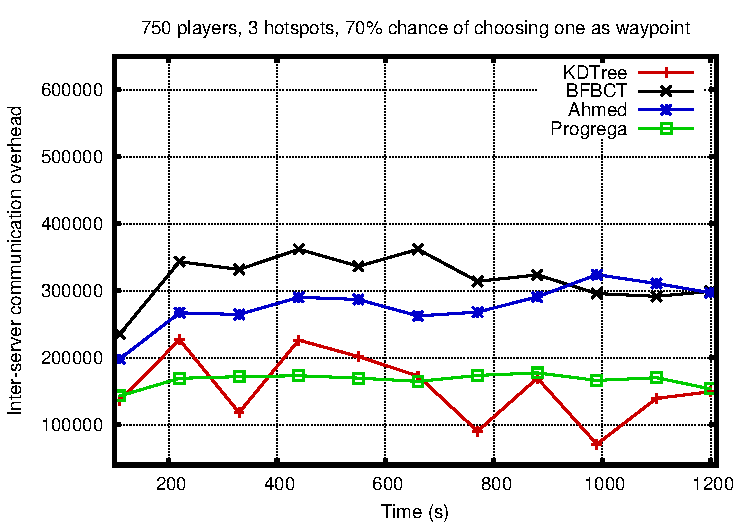
\includegraphics[width=0.49\linewidth]{data/750players_prob70/overhead}
	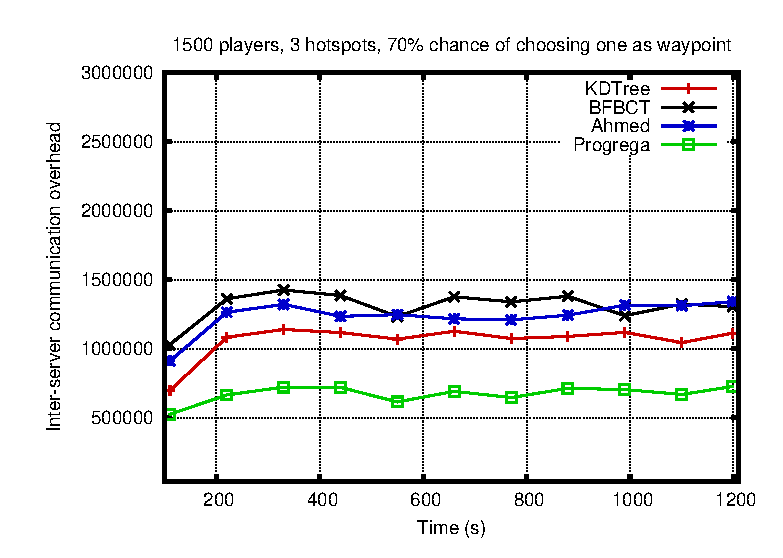
\includegraphics[width=0.49\linewidth]{data/1500players_prob70/overhead}
	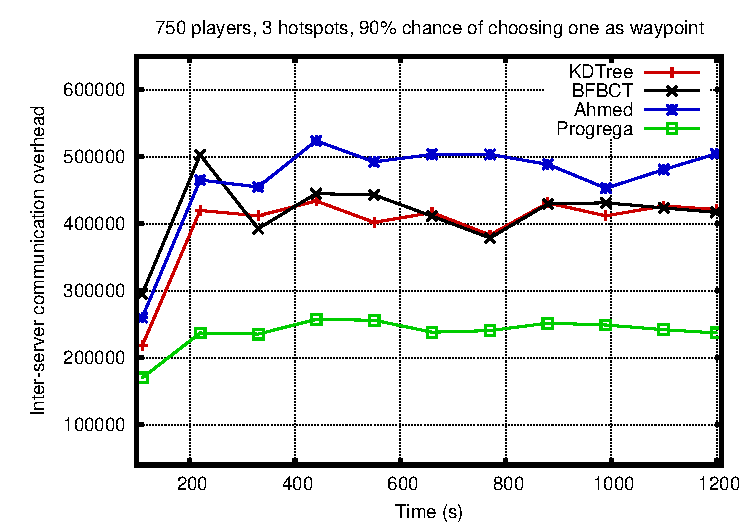
\includegraphics[width=0.49\linewidth]{data/750players_prob90/overhead}
	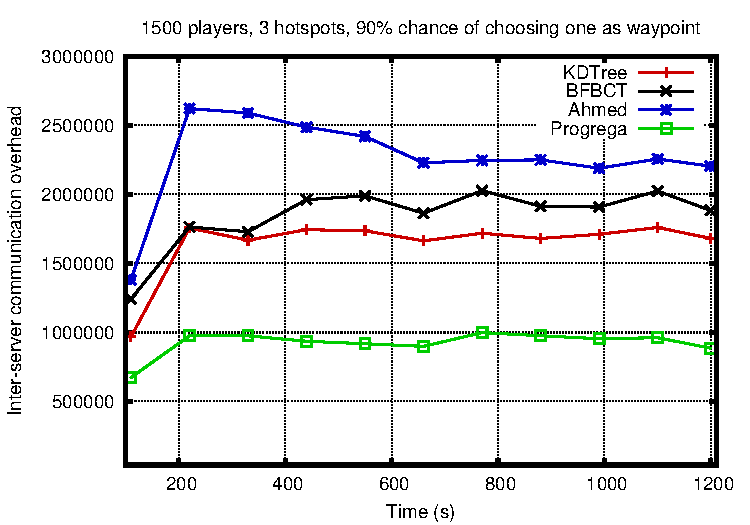
\includegraphics[width=0.49\linewidth]{data/1500players_prob90/overhead}

	\caption{Inter-server communication over time, for every algorithm in each scenario}
	\label{fig:overhead}
\end{figure}

Finally, it is shown the amount of communication between servers for each simulated algorithm, over time. As we can see in \figurecaption{} \ref{fig:overhead}, when there are no hotspots, the algorithm which uses the kd-tree is slightly better than the others. This is also explained by the fact that the regions are contiguous, minimizing the number of boundaries between them and, consequently, reducing the probability of occurring interactions between pairs of avatars, each one in a different region. However, it is also possible to see that the inter-server communication with Progrega was considerably lower than with the other algorithms in all the situations of system overload, except when there were 750 players with 70\% chance of an avatar moving to a hotspot, where Progrega and the kd-tree based algorithm alternated in the first place. The reason for this is that the main goal of Progrega -- besides balancing the load -- is precisely to reduce the communication between servers. However, even though it was not built specifically for reducing the overhead due to inter-server communication, the algorithm proposed here got second place overall in this criterion.

\section{Conclusions}
\label{sec:conc}

In this work, we proposed the use of a kd-tree to partition the virtual environment of MMOGs and perform the load balancing of servers by recursively adjusting the split coordinates stored in the nodes of the kd-tree. One of the conclusions reached was that the use of such data structures to make this partitioning allows a fine granularity of the load distribution, while the readjustment of the regions becomes simpler -- by recursively traversing the tree -- than the common approaches, based on cells and/or graph partitioning.

The finer granularity allows for a better balancing, so that the load assigned to each server is close to the ideal value that should be assigned to it. This better balance also helped to reduce the number of migrations, by performing less rebalancing operations. The fact that the regions defined by the kd-tree are necessarily contiguous was one of the factors that contributed to the results of the proposed algorithm, which was better than the other algorithms simulated in most of the criteria considered.

We have made an extensive set of simulations, comparing all the algorithms in six different scenarios, varying the number and distribution of avatars throughout the virtual environment of the game. By performing these tests, we have concluded that the proposed algorithm not only performs better than the others, but also that it scales better, at least in the kind of situations we considered, which we tried to make as close as possible to real MMOG scenarios -- although we defined very high load values in order to push the simulated algorithms and verify their behavior in worst case scenarios.

In conclusion, it was possible to use methods that can reduce the complexity of each rebalancing operation. This is due, first, to the reduction of the number of operations for calculating the relevance between pairs of avatars by sweeping a sorted avatar list and, second, to keeping at each server an avatar list already sorted in both dimensions, saving the time that would be spent on sorting the avatars when they were received by the server executing the rebalance.



\subsection{Acknowledgments}

The development of this work has been supported by the National Research Council (CNPq) and by the Coordination for Improvement of the Higher Education Personnel (CAPES).

\bibliographystyle{acmtrans}
\bibliography{kdtree}
\begin{received}
Received December 2009%;
%November 1993;
%accepted January 1996
\end{received}

%{\let\setcounter\mycounter
%	\elecappendix
%}

\medskip

\end{document}

